In this chapter we will briefly describe electronic voting in general, focusing mostly on the challenges and security parameters.

\section{Introduction}
In many aspects of our life's we in counter the act of voting, from simple things as voting whats for dinner, to the more complex things as a government election. The later involving a large number of people from different geographical locations. These election is normally handled by dividing the people into sections based on location, each section handling it's own sub-election and submitting the result to a overall tally. Though many countries still mostly rely on the old fashioned paper based ballots, we have in the recent years seen an increase in electronic voting. Electronic voting refers to the act of voting though an electronic devices and depending on the voting equipment and location, it can be divide into five categories \cite{Cet09}. 

\section{Classification}

\begin{description}
\item[DRE voting] Direct Recording Electronic is a specialized standalone electronic voting machine, which have the attributes of being physically hardened and have software specifically for voting installed. Votes casted on a DRE is do within a voting booth located on a polling site, and the votes is then recorded into a electronic ballot box.

\item[Poll-site voting] The voting is located on a polling site, votes are cast on public computers located on the site, in favour for voting booths. The computers on site are connected to a counting authority server though a closed and controlled network. Authentication can be done prior to the voting period or at the polling site

\item[Poll-site kiosk voting] Votes are casted inside a voting booth located at a polling site, using a terminal. The terminal is connected to a counting authority server though a closed and controlled network. Authentication is done at the polling site before allowed access to the voting booth. 

\item[Poll-site Internet voting] Votes are casted on public computers located on a polling site. The public computers on site is online and connected to a counting authority server over uncontrolled network. Authentication can be done prior to the voting period or at the polling site

\item[Remote Internet voting] Simply requires internet access and can be done from a home computer. Authentication is done prior to the voting an typical involves password or some type of authentication token. 

\end{description}


\section{The Voting Process}
Similar to the classification, there exist several of different systems and protocols for electronic voting. But they typically all follows the same process and includes the same actors as illustrated and describe below \cite{Cet09}. 

\begin{figure}[H]
\centering
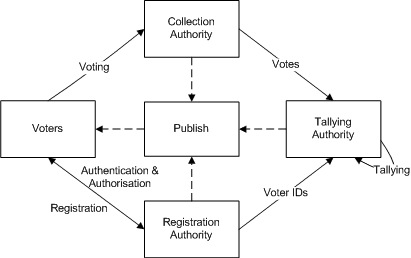
\includegraphics[scale=0.7]{Voting_Process.png}

\caption{Voting process}
\label{fig:Voting_Process}
\end{figure}

\begin{description}
    \item[Voter] Voter refers to a person who is eligible and who has registered for the privileges of voting in a given election. 
        
    \item[Registration authority] Registration authority refers to the authority that is responsible for registering eligible voters, and ensuring that only these voters are allowed to vote. Furthermore they ensures that voters only vote ones. 
        
    \item[Collection authority] The collection authority refers to the authority that is responsible for properly collecting all the votes. This authority can be represent as a simple electronic ballot box.

    \item[Tallying authority] Tallying authority are responsible for counting the votes of the election and publishing the result. 
\end{description}


\noindent
The voting process as illustrated on figure \ref{fig:Voting_Process} holds true for any voting system, and includes four stages. 

\begin{description}
    \item[Registration] Prior to an election, people who are eligible for voting, signs up to vote in the election. These voters are then registered, thus hereby ensuring no double voting acquires.
        
    \item[Authentication and Authorisation] Registered voters are authenticated, if they are found eligible and have not voted yet. Ones authenticated, the voter is giving access to cast his vote in the election.  
        
    \item[Voting] The voters cast there votes. 

    \item[Tallying] In this final stage the votes are counted, and of course only valid votes are being included. Ones the counting process is finished the final count is published. 
\end{description}


\section{Challenges}
Though the process of electronic voting have many similarities with paper based voting systems, there is still concern of the security. In paper based voting systems, the security is easily noticeable as this is represented by officials observing every stages of the process. the process typically goes along the lines of: When arriving to the polling site a voter typically already have proofs that he is eligible and is simply registered and handed the paper ballots. The paper ballot is fulfilled in a voting booth where only the voter himself is present. When fulfilled the ballot is folded or put in an envelope, in order to hide the vote is self, an then put in a ballot box located on the polling site. Note that ballot is anonymous and typical only requires a simple mark. Ones all the votes have been cast or a deadline is reached then the votes is counted. Throughout this entire process there are neutral officials physical present typically along with represents from each party in the election and passive observers.  

\noindent
In electronic voting systems the security is not this visible and if the system falls into the classification of \textit{Poll-site Internet voting} or \textit{Remote Internet voting} then uncontrolled network is used and the group of potential adversary is significantly increased.
To ensure security and public trust an electronic vote system should aim to fulfill the goals 
listed below \cite{Damgaard2003}

\begin{description}
    \item[Privacy] Throughout the process no information should be leaked, only the final counting
    should be made public. At no time should a vote could be linked to the voter. 
    
    \item[Robustness] The system should be tolerant against cheating. Only valid and correctly fulfilled ballots should be counted. Nobody should be able to manipulating the final count.

    \item[Universal verifiability] The final count should be public verifiable. Anyone should be able to convince himself of the fairness of the election. This should be done without gain any other information.
        
\end{description}

\section{Security Requirements}
The previous three goals are fairly board and can with benefit be specified into concrete security requirements as done in \cite{Cet08}

\begin{itemize}
    \item \textit{Voter Privacy}
        No one should be able to link a vote back to the specific voter, and only the voter should
        know his vote. These requirements shall hold during and after the election.  
    
    \item \textit{Eligibility}    
        Only Eligible and registered voters can vote. 
    
    \item \textit{Uniqueness}
        Only one vote per registered voter should be counted.
    
    \item \textit{Fairness}
        None should be able to gain any knowledge of the outcome of the election, before the ending. This is to prevent voters of voting accordingly to any leaked information. 
    
    \item \textit{Uncoercibility}
        Nobody should be able to extract the value of a vote. This is to prevent anybody from compelling a voter by force, intimidation, or authority to cast a vote in a specific way. 
    
    \item \textit{Receipt-freeness} 
        The voting system should not produce a receipt that reveals any information about the casted vote. This is to prevent a vote from trading his vote. 
    
    \item \textit{Accuracy} 
        The final tally should be correctly computed from valid casted votes. It should not be
        possible to manipulate the final tally without being detected. 
    
    \item \textit{Universal Verifiability}
        It should be possible for any participants and observers to validate individual votes as well as the final tally of the election. 
    
    \item \textit{Individual Verifiability}    
        Every registered voter should be able to verify that his vote is counted correctly. 
    
\end{itemize}


\section{Approaches}
To construct a electronic voting system that fulfills these security requirements, we look that three fundamentally different approaches 

\begin{description}
    \item[Blind signatures]

    \item[Mix-nets]        
        
    \item[Homomorphic encryption]
\end{description}

This that are to be detailed in this chapter: 

\begin{description}
    \item[Voter]
    \item[Tallier]
    \item[Observer]
    \item[Bulletin board]
\end{description}